\documentclass[12pt]{article}

\usepackage{amsmath}
\usepackage{amssymb}
\usepackage{graphicx}
\usepackage{epstopdf}
\usepackage{inputenc}
\usepackage{geometry}
\geometry{left=2.5cm,right=2.5cm,top=2.5cm,bottom=2.5cm}
\begin{document}

\title{UniGuideOnline \\ }

\author{William Hadden - 6249537} 

\maketitle

\section*{Introduction}

% motivation 

% idea (what is the app)

%bit about aws 

\section*{Application}
\section{Architecture}

This application follows the design principles of a 3-tier architecture. Namely, there are webservers that handle incoming client traffic and display page information, a backend database server for handling application specific data and an API that links them together.

There are two webservers, installed on EC2 instances that both host React applications. One webserver (the public-webserver) takes care of displaying paper information in a dashboard like style which the other (admin-webserver) provides functionality for paper providers; for example, academics to create papers. The backend database is provisioned by DynamoDB, a managed NoSQL database provided by AWS. Finally, there is a CRUD API created using a combination of API Gateway which provides routes and endpoints, coupled with a lambda function that executes custom code in response to requests from the API Gateway. 

\begin{figure}
    \caption{Diagram of application architecture.}
    \label{fig: application_architecutre}
    % \includegraphics[]{} 
\end{figure}

% ec2 instances 
Each webserver is hosted on a customized EC2 instance. A key part of the design is splitting the two different user interactions - that of a paper viewer and paper administrator - onto separate virtual machines. The idea is that the traffic demands on either will almost certainly be different. For example, there are certainly more students than academics at regular universities. As such, we would expect the traffic on the user oriented webservers to be higher. Therefore, this separation of concerns allows more or less instances to be brought online in response to differential traffic/demand. This could be accomplished using a load balancer in the future. In essence, this separation makes it easy to tweak individual provisioning to match the demand. 
Furthermore, anticipating this extension, both EC2 instances use pm2 software installed to automatically run their respective webservers on restart. 

Each instance is also associated with an elastic IP. The idea here again relates to the load balancing with the operation of multiple instances where the elastic IPs can mask the failures of instances by instant remapping the address to other running instances. Furthermore, upon acquiring a domain name, this can ensure that the domain points to the instance(s).

% API
The API is provisioned using a combination of an API Gateway and a lambda function. The key idea here is running code only on demand. In this instance, the API Gateway service is always visible and able to be accessed. However, the lambda function only runs the code required to accomplish the request when the endpoint is triggered, thereby saving money.   

% Database
The database backend is provided by the DynamoDB service. This service greatly simplifies the backend logic since AWS takes care of all the particulars. Thus, all that is required is the correct triggering of the provided API. 

\section{Data Model}
The database consists of a single collection named papers.

\begin{figure}
    \caption{Paper collection data model.}
    \label{fig: paper_data_model}
    \begin{center}
        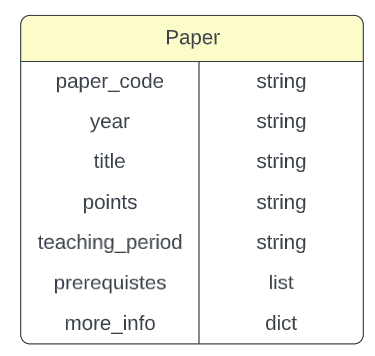
\includegraphics[width=0.2\textwidth]{../docs-assets/paper_erd.PNG}
    \end{center}
\end{figure}

Note that the paper objects can refer to other paper objects. In this case, I opted for a NoSQL database because it more easily links with the graph structure I wanted to accomplish with the paper structures. While some recent RDBMSs do offer tree structures without significant slowdown, I determined that in this case, with the small workload I am anticipating, it is simply easier and less logically intense to use a simple document oriented NoSQL database.

\section*{LifeCycles}

\section{Initial setup}

\section{Development}

\section*{Estimated costs of cloud services}
\section*{User Interaction}

\section*{Development story}

% terraform 
Spent a lot of time trying to get to work.
Basically was defeated by the IAM role that had to be assigned to certain resources would lead t me being either locked out of certain functionality (i.e I couldn't see my functions on the AWS GUI) and to terraform destroy failing because the IAM user couldn't be deleted with it.

(The lambda function required an execution role)
%ec2 


%API
Clearly I was always going to need a nice way to interact with the different components. I decided to have a serverless function so that I didn't have to run another virtual machine which would be both expensive, slow and difficult to maintain (especiialy without CI/CD)

% CI/CD
Would make the startup and development some much faster and nicer. However, learner labs don't support it


% eventual outcome


\section*{Cloud specific information}

% estimation of running costs

% idle

% with light use

\section*{Future improvements}

% CI/CD
Not possible with learner lab so would need own account but would make this application x100 better

% Authorization control/user accounts for managing data
Creation of user accounts such that the privileges for interacting with resources (such as papers) can be restricted, so only their owners can interact with them

% cloud front network
Use of a CDN and load balancing would increase the reliability of the app and allow it to scale out 

% terraform
Would like to have another go at this but again, doens't really work with learner lab

% connect the two togehter with references 
Href into either through a authenication/user dialog to better increase the app 

% inclusion of scrapers

\end{document}